\setcounter{figure}{0}
\setcounter{lstlisting}{0}
\section{Vježba 4: SURF}

\subsection{Opis vježbe}
Izraditi 2D model nekog objekta na temelju slike tog objekta snimljenog
kamerom. Razmatrani model predstavlja skup 2D točaka detektiranih
SURF-metodom kojima su pridruženi lokalni deskriptori. Potrebno je
raspoznati objekt na drugoj slici koja je također snimljena kamerom, ali
iz drugog položaja.  
\\
\begin{lstlisting}[language=bash,caption={Pokretanje programa iz
    komandne linije}]
$ ./feature_matching ../images/sm-object.jpg ../images/sm-scene.jpg 
\end{lstlisting}

\subsection{Objašnjenje programa}

\subsubsection{Kontrola programa}

Prilikom pokretanja programa iz komandne linije potrebno je 
predati programu putanju do slike objekta (argv[1]) i putanju do slike
scene (argv[2]). 
\\

\begin{lstlisting}[language=C,caption={Kontrola programa tipkovnicom}]
while (1){
    char c = waitKey(10);
    switch(c) {
            case 's':
                surfFlannMatcher ();
                break;
\end{lstlisting}

\newpage
\subsubsection{SURF}

\begin{lstlisting}[language=C,caption={Detekcija objekta na drugoj
    slici}]
void surfFlannMatcher ()
{
    Mat imgObject = imread (globalArgv[1], CV_LOAD_IMAGE_GRAYSCALE);
    Mat imgScene = imread (globalArgv[2], CV_LOAD_IMAGE_GRAYSCALE);
    if (!imgObject.data || !imgScene.data) { 
      cout<< "Error reading images " << endl; 
      return; 
    }

    // Threshold for the keypoint detector. Only features, 
    // whose hessian is larger than minHessian are 
    // retained by the detector. Therefore, the larger the
    // value, the less keypoints you will get.
    int minHessian = 400;
    // Detect the keypoints using SURF Detector
    SurfFeatureDetector detector(minHessian);
    vector<KeyPoint> keypointsObject, keypointsScene;

    // Detection of object and scene keypoints (location, 
    // diameter of the meaningful keypoint neighborhood)
    detector.detect (imgObject, keypointsObject);
    detector.detect (imgScene, keypointsScene);
    cout << "Number of keypoints in object: " << 
        keypointsObject.size() << endl;
    cout << "Number of keypoints in scene: " << 
        keypointsScene.size() << endl;

    // Calculate descriptors (feature vectors)
    // on detected keypoints
    SurfDescriptorExtractor extractor;
    Mat descriptorsObject, descriptorsScene;
    extractor.compute (imgObject, keypointsObject, descriptorsObject);
    extractor.compute (imgScene, keypointsScene, descriptorsScene);

    // Matching descriptor vectors using FLANN matcher
    // Fast approximate nearest neighbor
    FlannBasedMatcher matcher;
    // DMatch - Class for matching keypoint descriptors
    vector<DMatch> matches;
    matcher.match (descriptorsObject, descriptorsScene, matches);

    double maxDist = 0; double minDist = 100;
    // Quick calculation of max and min distances between keypoints
    for( int i = 0; i < descriptorsObject.rows; i++ ) { 
        double dist = matches[i].distance;
        if( dist < minDist ) minDist = dist;
        if( dist > maxDist ) maxDist = dist;
    }
    // Class for matching keypoint descriptors: 
    // query descriptor index, train descriptor index, 
    // train image index, and distance between descriptors.
    vector<DMatch> goodMatches;
    // Draw only "good" matches (i.e. whose distance is 
    // less than 3*minDist )
    for( int i = 0; i < descriptorsObject.rows; i++ )
    { if( matches[i].distance < 3*minDist )
     { goodMatches.push_back( matches[i]); }
    }

    Mat imgMatches;
    // Draws only paired keypoints with random colors
    drawMatches (imgObject, keypointsObject, imgScene, keypointsScene,
               goodMatches, imgMatches, Scalar::all(-1), 
               Scalar::all(-1), vector<char>(), 
               DrawMatchesFlags::NOT_DRAW_SINGLE_POINTS);

    // Localize the object
    vector<Point2f> obj;
    vector<Point2f> scene;
    for (int i = 0; i < goodMatches.size(); i++) {
    // Get the keypoints location from the good matches
    obj.push_back (keypointsObject[ goodMatches[i].queryIdx ].pt);
    scene.push_back (keypointsScene[ goodMatches[i].trainIdx ].pt);
    }
    // Finds a perspective transformation between two planes.
    // Using RANSAC method
    Mat H = findHomography (obj, scene, CV_RANSAC);

    // Get the corners from the image1 (the object to be "detected")
    vector<Point2f> objCorners(4);
    objCorners[0] = cvPoint (0,0); 
    objCorners[1] = cvPoint (imgObject.cols, 0);
    objCorners[2] = cvPoint (imgObject.cols, imgObject.rows); 
    objCorners[3] = cvPoint (0, imgObject.rows);
    vector<Point2f> sceneCorners(4);

    // Perfom perspective transform 
    perspectiveTransform (objCorners, sceneCorners, H);
    // Draw lines between the corners 
    // (the mapped object in the scene - image2)
    line (imgMatches, sceneCorners[0] + Point2f (imgObject.cols, 0), 
            sceneCorners[1] + Point2f (imgObject.cols, 0), 
            Scalar(0, 255, 0), 4);
    line (imgMatches, sceneCorners[1] + Point2f (imgObject.cols, 0), 
            sceneCorners[2] + Point2f (imgObject.cols, 0), 
            Scalar( 0, 255, 0), 4);
    line (imgMatches, sceneCorners[2] + Point2f (imgObject.cols, 0), 
            sceneCorners[3] + Point2f (imgObject.cols, 0), 
            Scalar( 0, 255, 0), 4);
    line (imgMatches, sceneCorners[3] + Point2f (imgObject.cols, 0), 
            sceneCorners[0] + Point2f (imgObject.cols, 0), 
            Scalar( 0, 255, 0), 4);
    // Show detected matches
    imshow ("Good Matches & Object detection", imgMatches);
    waitKey(0);
}
\end{lstlisting}

\begin{figure}[h]
\centering
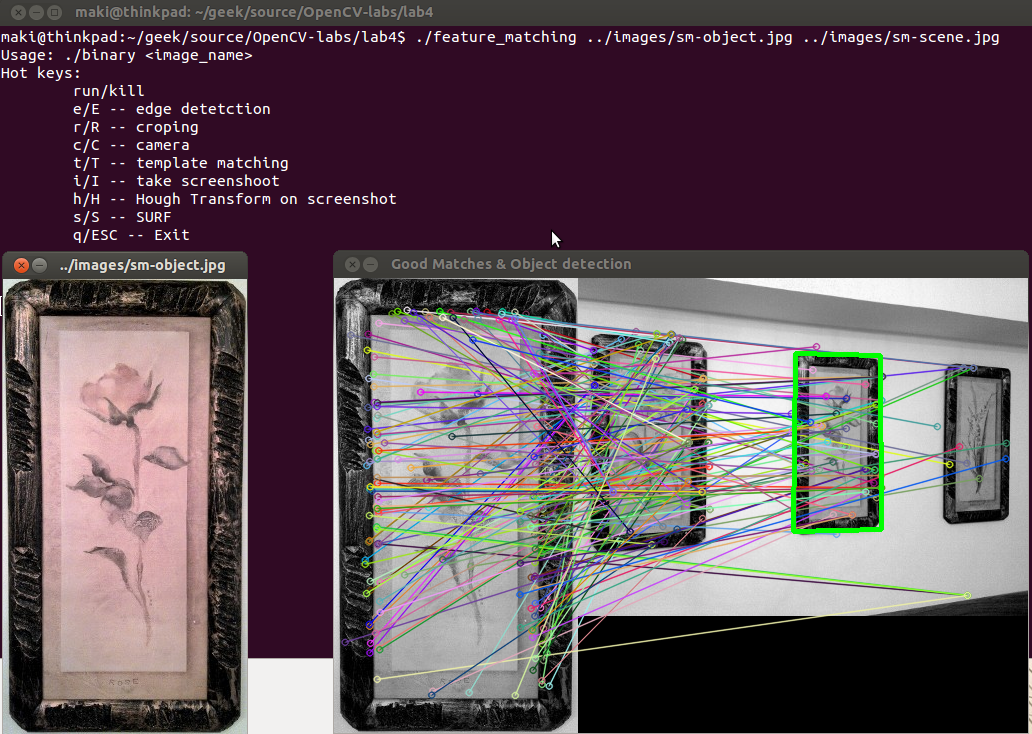
\includegraphics[scale=0.42]{images/lab4-surf-01.png}
\caption{SURF - pronalazak objekta u sceni}
\label{fig:lab4-surf-01}
\end{figure}

\newpage
\subsection{Zaključak}
Cilj ove vježbe bio je izrađeni 2D model objekta prepoznati na 
slici koja je snimljena iz drugog položaja.
To smo postigli koristeći SURF (engl. \textit{Speeded Up Robust
Features} metodu za određivanje značajki. Prvo smo pomoću
\textit{SurfFeatureDetector()} klase detektirali ključne točke
objekta i scene. Zatim smo koristeći \textit{SurfDescriptorExtractor()}
klasu pronašli značajke ključnih točaka objekta i scene. Zatim smo
sparili značajke ključnih točaka objekta i scene. Na kraju smo prikazali
samo one točke kojima smo pronašli par te smo nacrtali dužine između
sparenih parova točaka.
\\
Slika koju smo koristili za testiranje je pažljivo odabrana jer se radi
o sličnim crtežima različitih cvijetova. Također treba primjetiti
da slike imaju slične ali različite okvire. Te smo upravo na ovakvom
primjeru pokazali spospobnosti SURF algoritma za detekciju značajki.
\\
Programi koji detektiraju i opisuju značajke te su još neovisni o
rotaciji i veličini objekta kojeg opisuju imaju veliki značaj u
aplikacijama koje se bave detekcijom objekata. Ove metode su isto tako
dosta otporne na šum i promjenu osvijetljenja. 

